%%\subsection{Re-weighting for the tagging jets}
\label{subsec:mjj_reweight}
\label{subsec:mjj_reweight_1lep}

This section examines the modeling of the \Wjets background for the 1-lepton channel, focusing on the mismodeled invariant mass of the two selected Tag Jets (\mjjtag) in the Sherpa 2.2.1 \Vjets samples. The forward topology of our final state makes \mjjtag a critical variable. To address the observed mismodeling, we applied a linear reweighting procedure to the \Wjets MC samples, ensuring alignment with data in the CRs. 
Figure~\ref{fig:mjjReweight1LepMjjDistBefore} illustrates the \mjjtag distributions for both merged and resolved regions, highlighting the noticeable discrepancies between the primary background source and the observed data.

To correct the mismodeling, which we assume varies linearly with \mjjtag, we apply the following reweighting formula to the \Wjets events:
\begin{equation}
  w(m_{jj}^{tag}) =  p_0 + p_1 \cdot m_{jj}^{tag} ,
\end{equation}
%
where $p_0$ and $p_1$
are coefficients calculated independently for both merged and resolved regions.
The function $w(m_{jj}^{tag})$ represents the weight adjustment applied to each event, modifying the original event weight based on the \mjjtag value.
After determining these coefficients from CRs (see Table~\ref{tab:mjjReweight1LepRegions}), we apply the corrections to the respective SRs. 
For both merged and resolved scenarios, $p_0$ and $p_1$ are obtained by fitting the Sherpa \Wjets model-to-data ratio, after subtracting non-\Wjets backgrounds.

In the merged case, a single fit is applied to the entire \mjjtag distribution without subdividing the sample based on the $m_{J}$ range. This approach not only simplifies the analysis but also maintains statistical robustness, as illustrated in Figure~\ref{fig:mjjReweight1LepMer}.

In the resolved case, the fit to \mjjtag is performed within specific $m_{jj}^{sig}$ bins ([50, 60, 70, 100, 120, 150, 200, 300] GeV), excluding the [70, 100] GeV bin as it corresponds to the resolved signal region and we aim to fit using only control region data.
This approach segments both MC and data samples according to $m_{jj}^{sig}$, as illustrated in Figure~\ref{fig:mjjReweight1LepResPtBins}. Subsequently, the parameters $p_0$ and $p_1$ are determined across these bins. These parameters are then fitted to define the definitive reweighting factors for the signal region's $m_{jj}^{sig}$, as shown in Figure~\ref{fig:mjjReweight1LepResFit}. An interpolation from the control to the signal region follows this step.

The study encompasses all data periods and corresponding MC campaigns (mc16a, mc16d, and mc16e). To verify consistency across various data periods and pileup conditions, these analyses were independently repeated for each MC campaign. The outcomes are presented in Figure~\ref{fig:mjjReweight1LepResTotal}. Although a slight dependence on the MC period was observed, the benefits of adjusting the \mjjtag reweighting for each period proved to be minimal. Thus, the combined period results were utilized for the final analysis.

Table~\ref{tab:1lepReweighting} shows the final parameters derived for the \olep channel.
The \mjjtag distributions for the three SRs before and after reweighting are depicted in Figures~\ref{fig:mjjReweight1LepMjjDistBefore} and \ref{fig:mjjReweight1LepMjjDistAfter}, respectively.

\begin{table}[ht]
    \centering
    \caption{Definition of control regions used to derive \Wjets reweighting factors.}
    \begin{tabular}{|c|c|}
        \hline
        \multirow{2}{4em}{Resolved} & pass Resolved Selection (NoMassWindowCut)  \\
         & BjetVeto  \\
         \hline
        \multirow{2}{4em}{Merged} &  pass Merged Selection (NoMassWindowCut) \\
        & BjetVeto  \\
         \hline
    \end{tabular}
%    \caption{Definition of control regions used to derive \Wjets reweighting factors.}
    \label{tab:mjjReweight1LepRegions}
\end{table}

%%Table ~\ref{tab:1lepReweighting} shows the final parameters derived for the \olep channel.

\begin{table}[ht]
\centering
\caption{1-lepton $m(jj)^\text{tag}$ reweighting factors.}
\label{tab:1lepReweighting}
\begin{tabular}{ |c|c|c| }
\hline
Parameter & Merged CRVjet & Resolved CRVjet  \\
\hline
$p_{0}$ (slope) [$\GeV^{-1}$] & $(-51.4 \pm 2.9)10^{-5}$ &  $(-14.4 \pm 6.1)10^{-5}$ \\
 \hline
$p_{1}$ (constant)  & $1.47 \pm 0.03$ & $1.13 \pm 0.02$ \\
\hline
\end{tabular}
\end{table}

\clearpage
\begin{figure}[ht]
    \centering
    \begin{subfigure}[b]{0.3\textwidth}
        \centering
        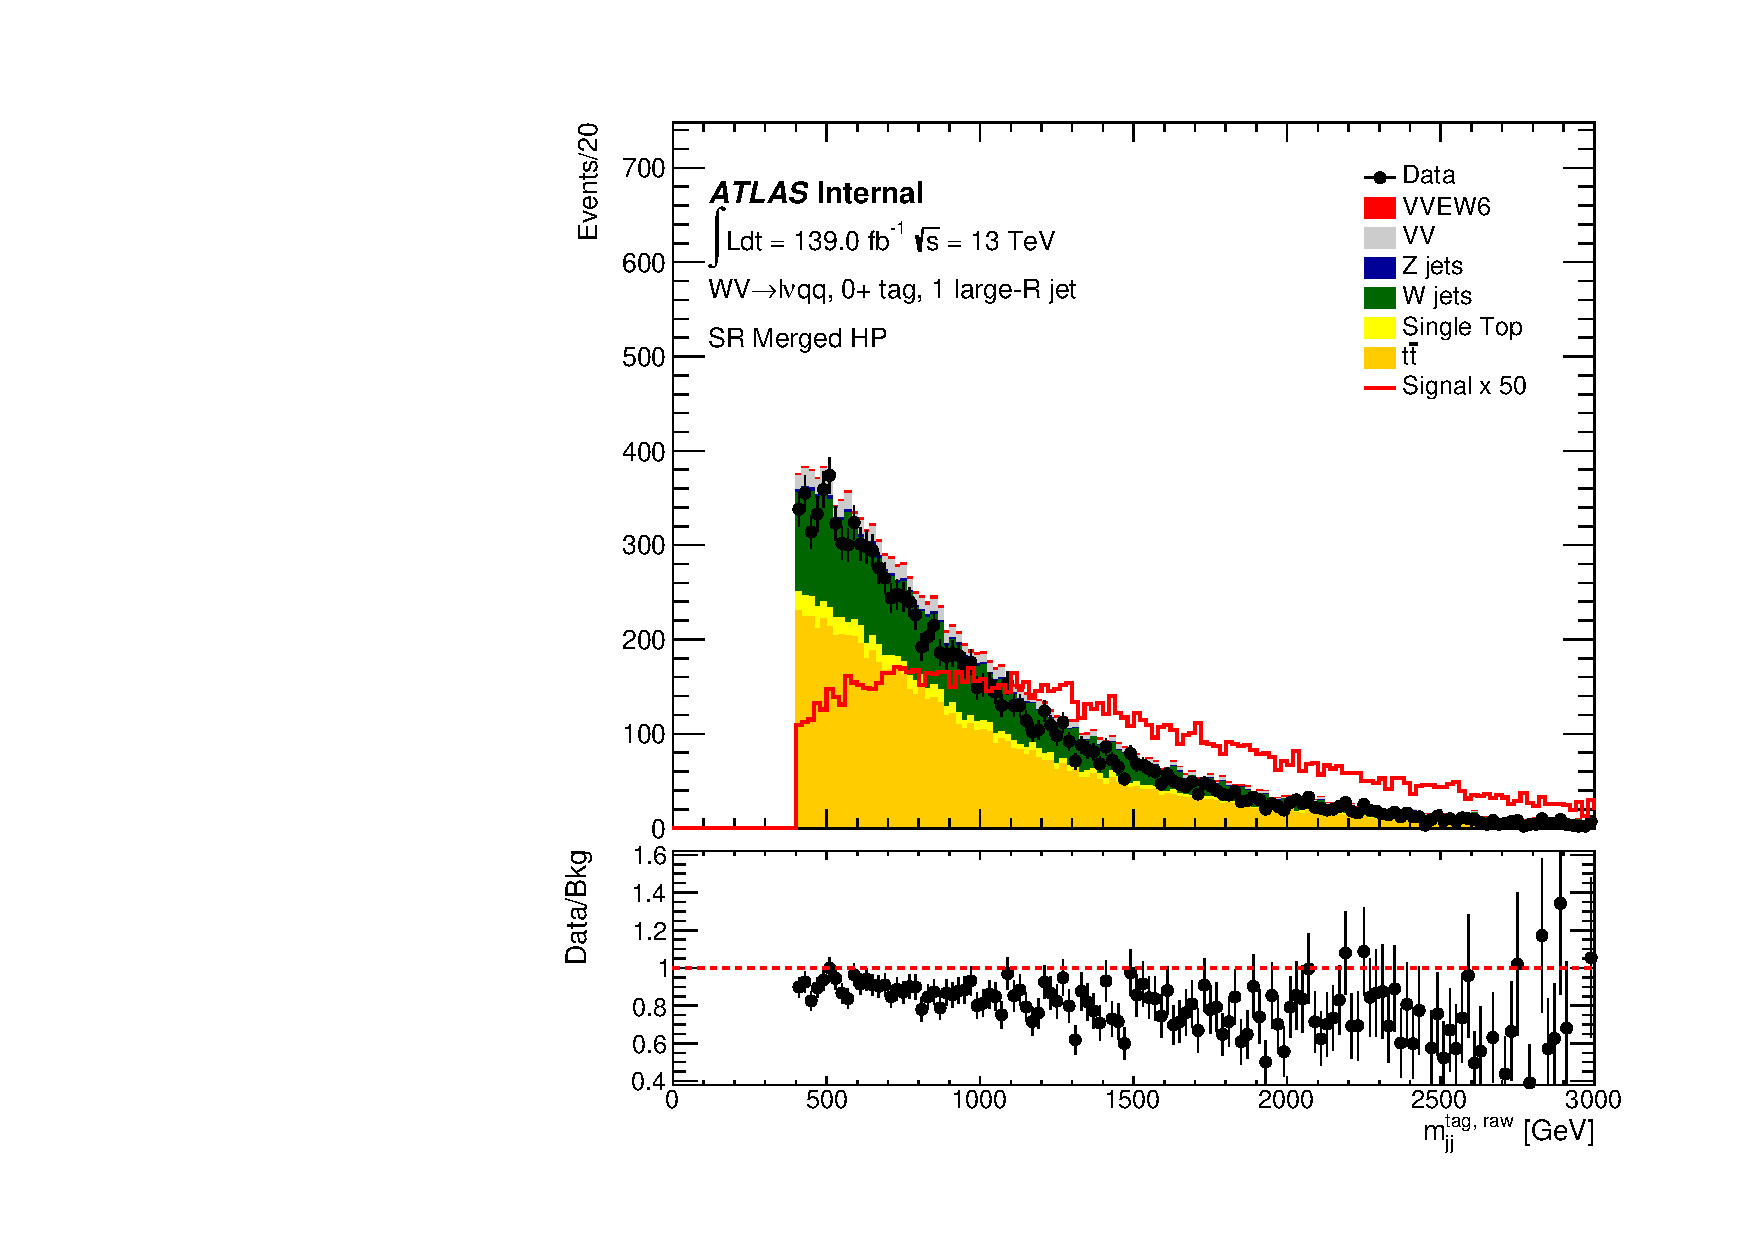
\includegraphics[width=\textwidth]{figures/mjjreweight1lep/SR_50/stacked_plot_merged_tagMjj_MjjWeightMerged.pdf}
        \caption{Merged HP SR RAW}
        \label{fig:MC16ADE_Merged_HP_SR_Before}
    \end{subfigure}
    \hfill
    \begin{subfigure}[b]{0.3\textwidth}
        \centering
        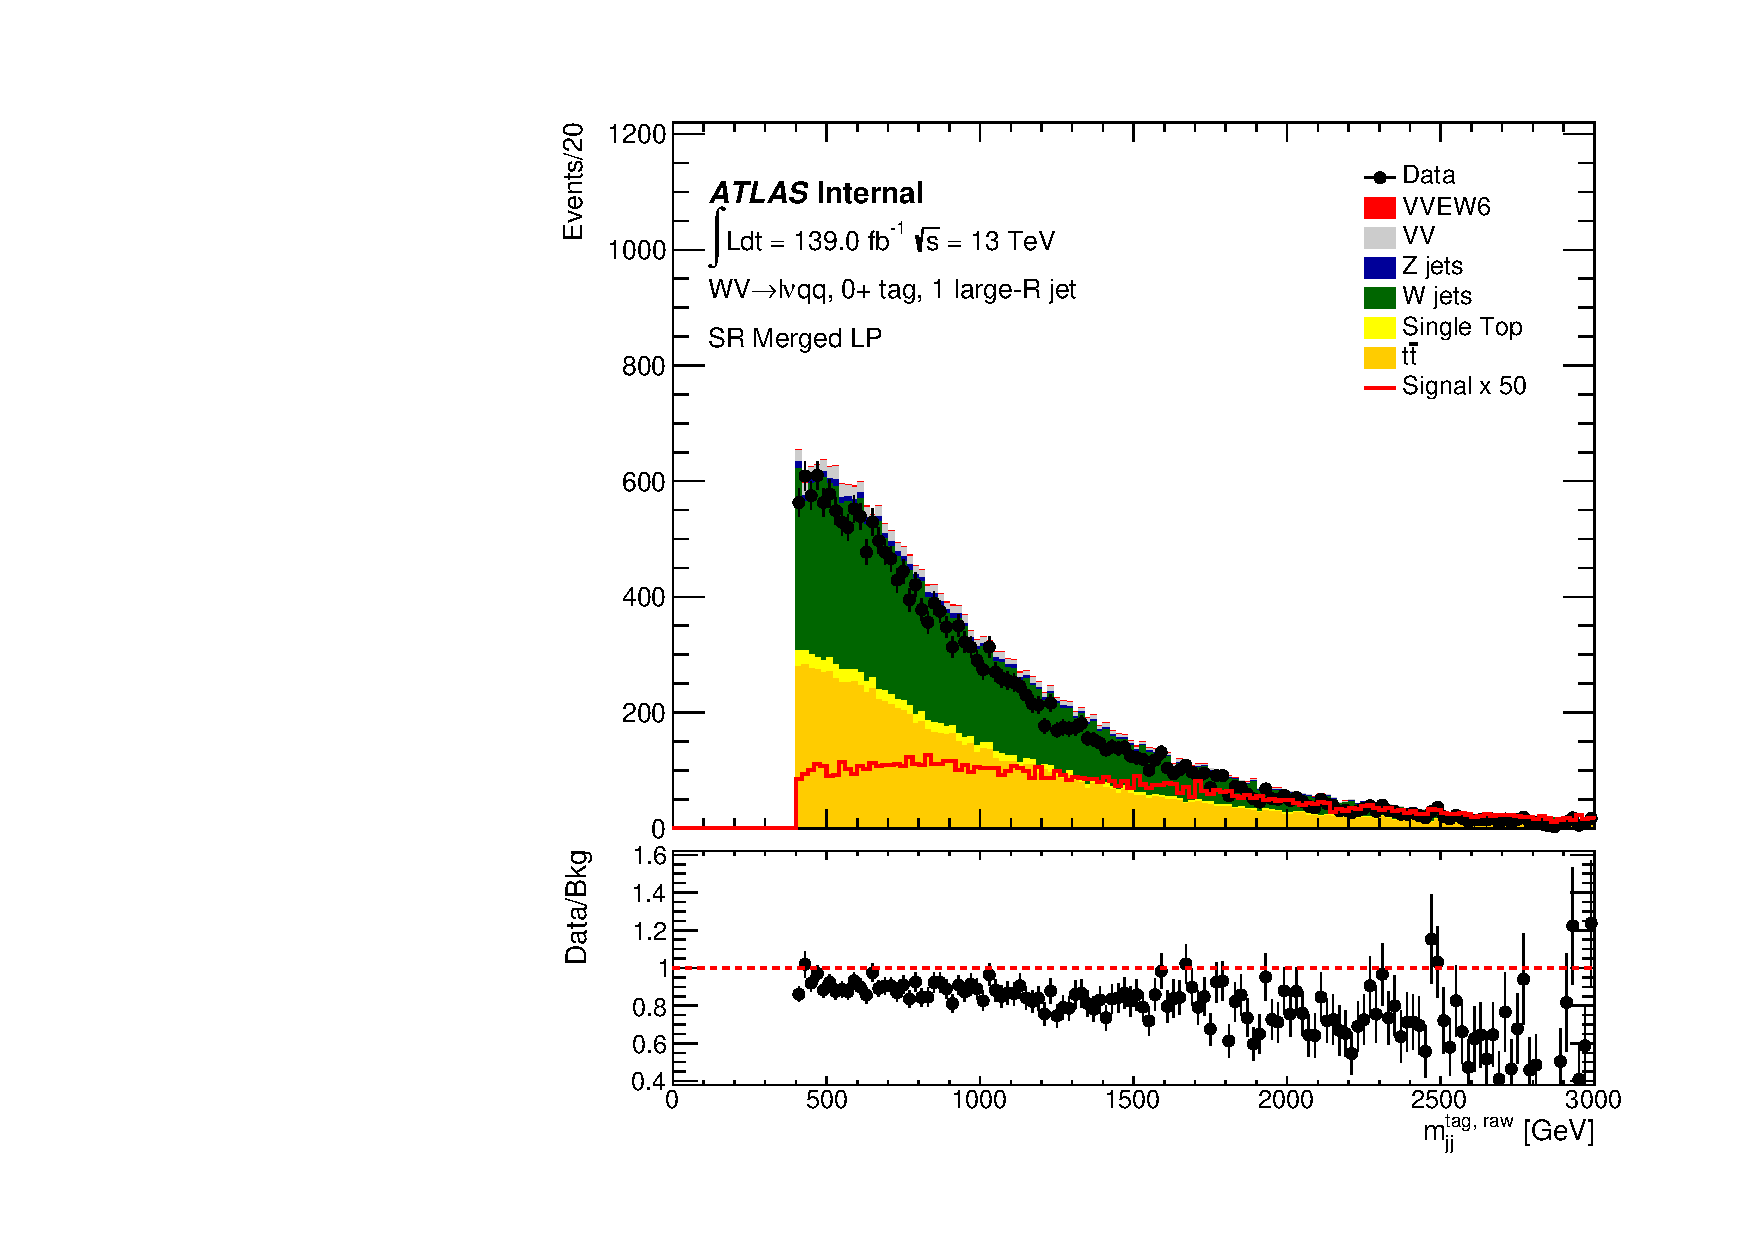
\includegraphics[width=\textwidth]{figures/mjjreweight1lep/SR_80/stacked_plot_merged_tagMjj_MjjWeightMerged.pdf}
        \caption{Merged LP SR RAW}
        \label{fig:MC16ADE_Merged_LP_SR_Before}
    \end{subfigure}
    \hfill
    \begin{subfigure}[b]{0.3\textwidth}
        \centering
        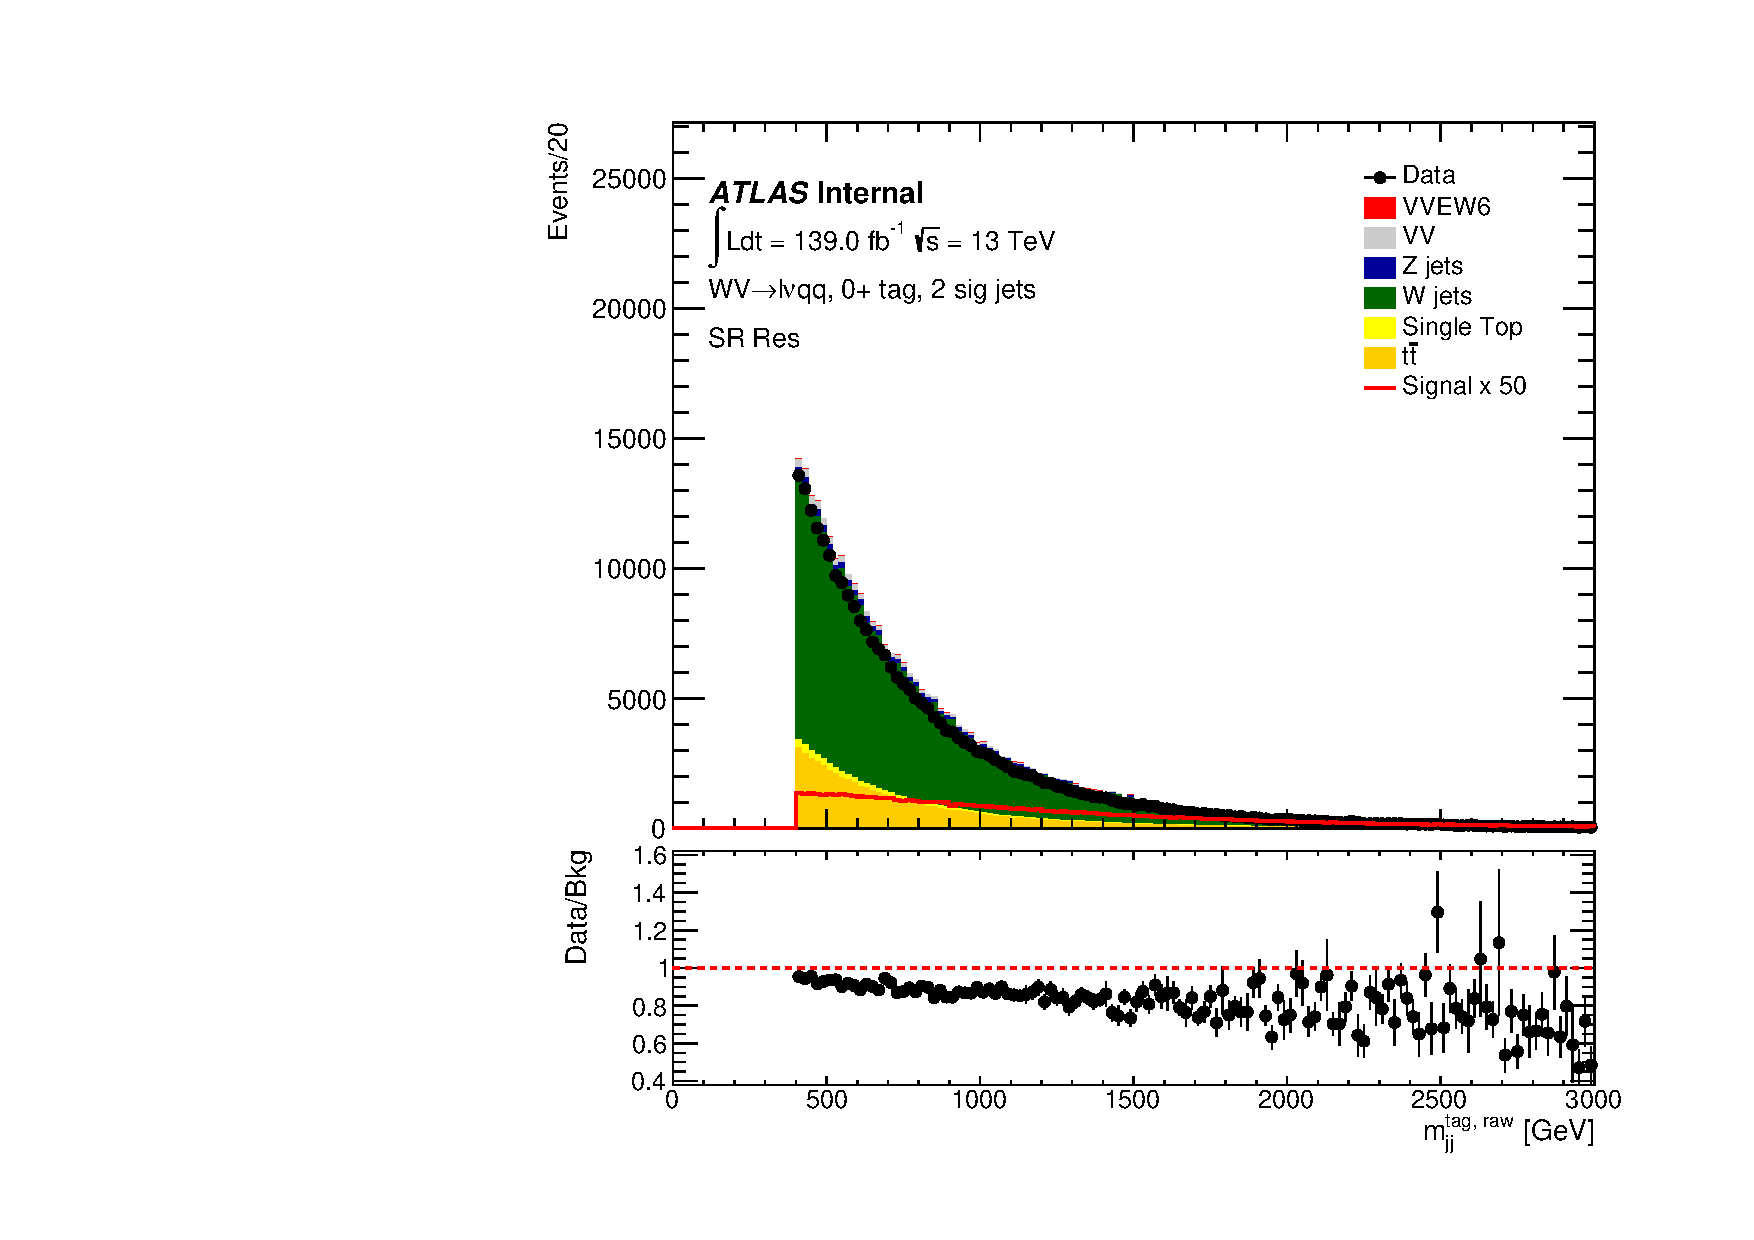
\includegraphics[width=\textwidth]{figures/mjjreweight1lep/SR_Res/stacked_plot_resolved_tagMjj_MjjWeightResolved.pdf}
        \caption{Resolved SR RAW}
        \label{fig:MC16ADE_Resolved_SR_Before}
    \end{subfigure}
    \caption{\mjjtag distributions without any corrections in the signal regions.}
    \label{fig:mjjReweight1LepMjjDistBefore}
\end{figure}

\begin{figure}[ht]
    \centering
    \begin{subfigure}[b]{0.3\textwidth}
        \centering
        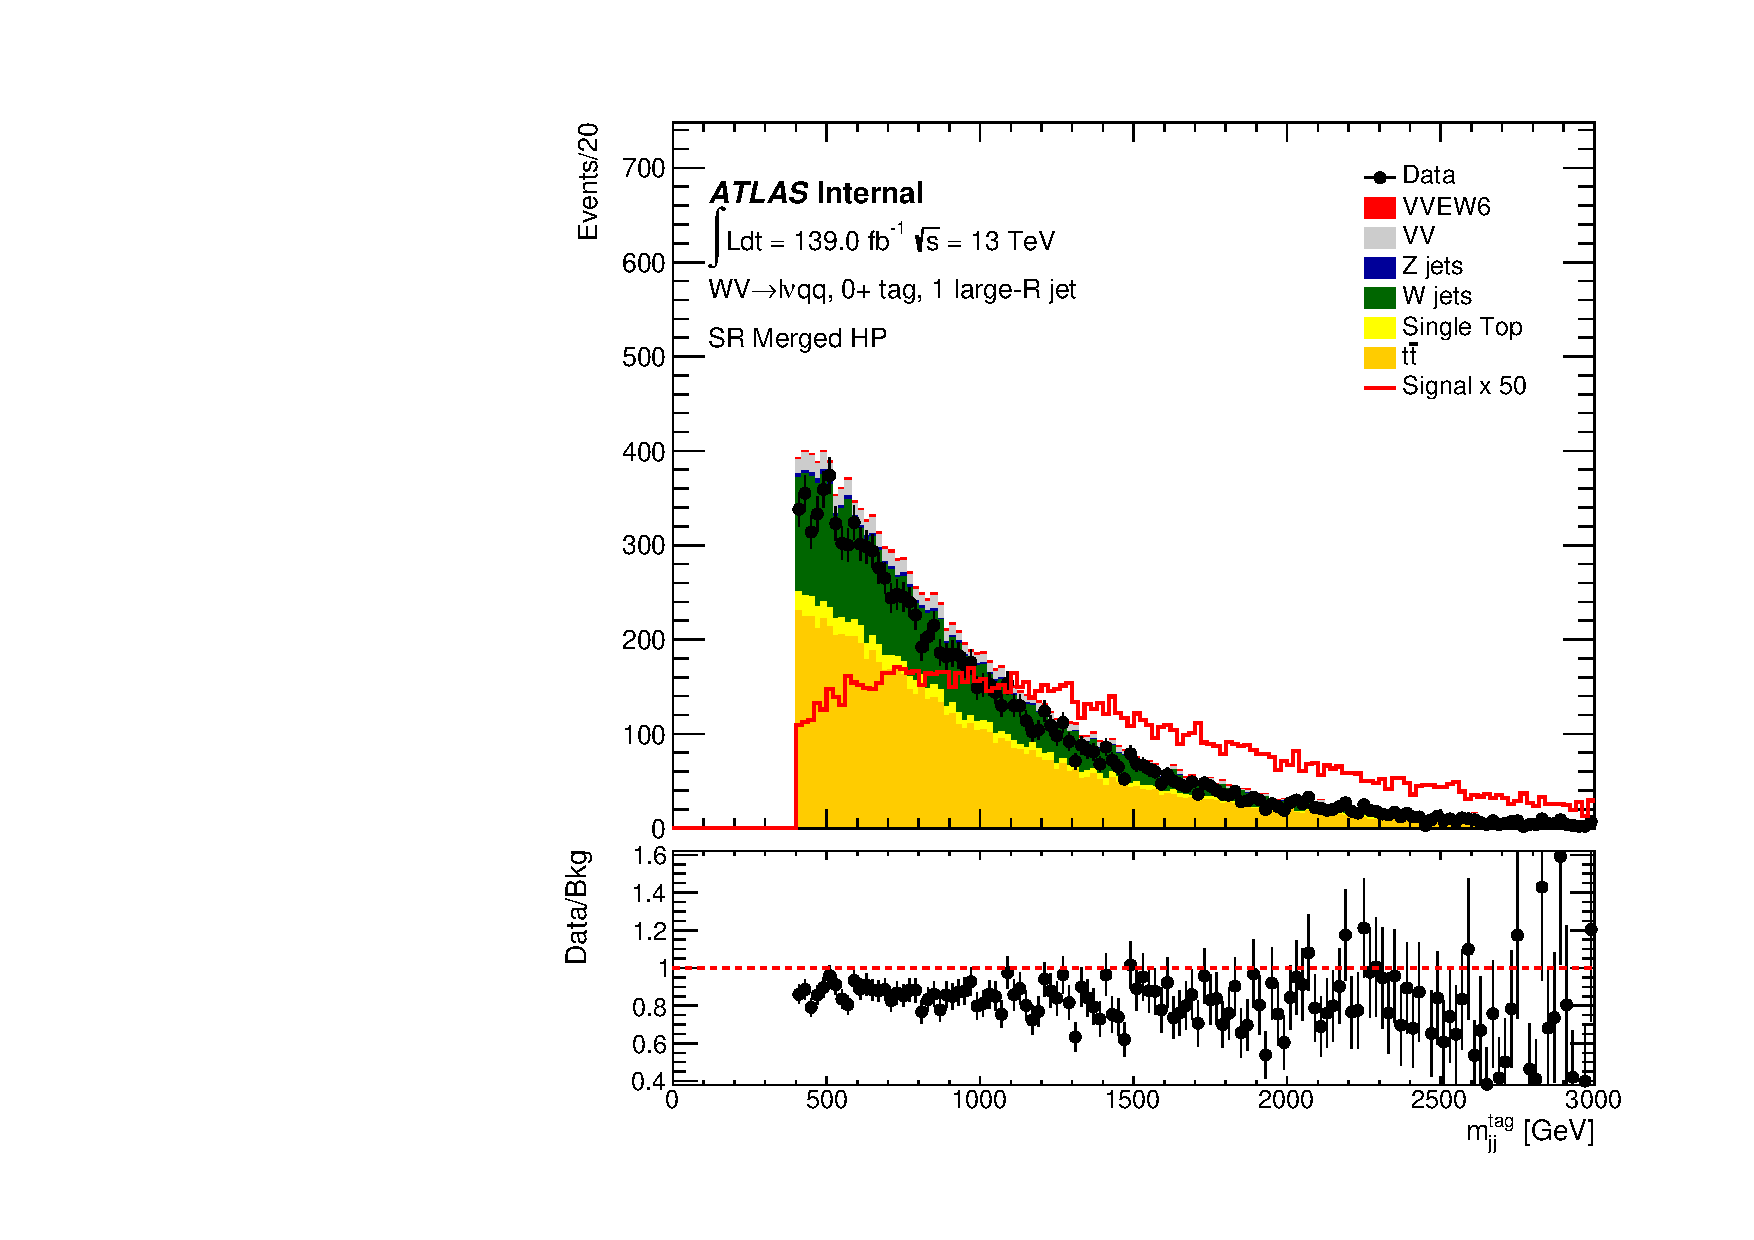
\includegraphics[width=\textwidth]{figures/mjjreweight1lep/SR_50/stacked_plot_merged_tagMjj.pdf}
        \caption{Merged HP SR}
        \label{fig:MC16ADE_Merged_HP_SR}
    \end{subfigure}
    \hfill
    \begin{subfigure}[b]{0.3\textwidth}
        \centering
        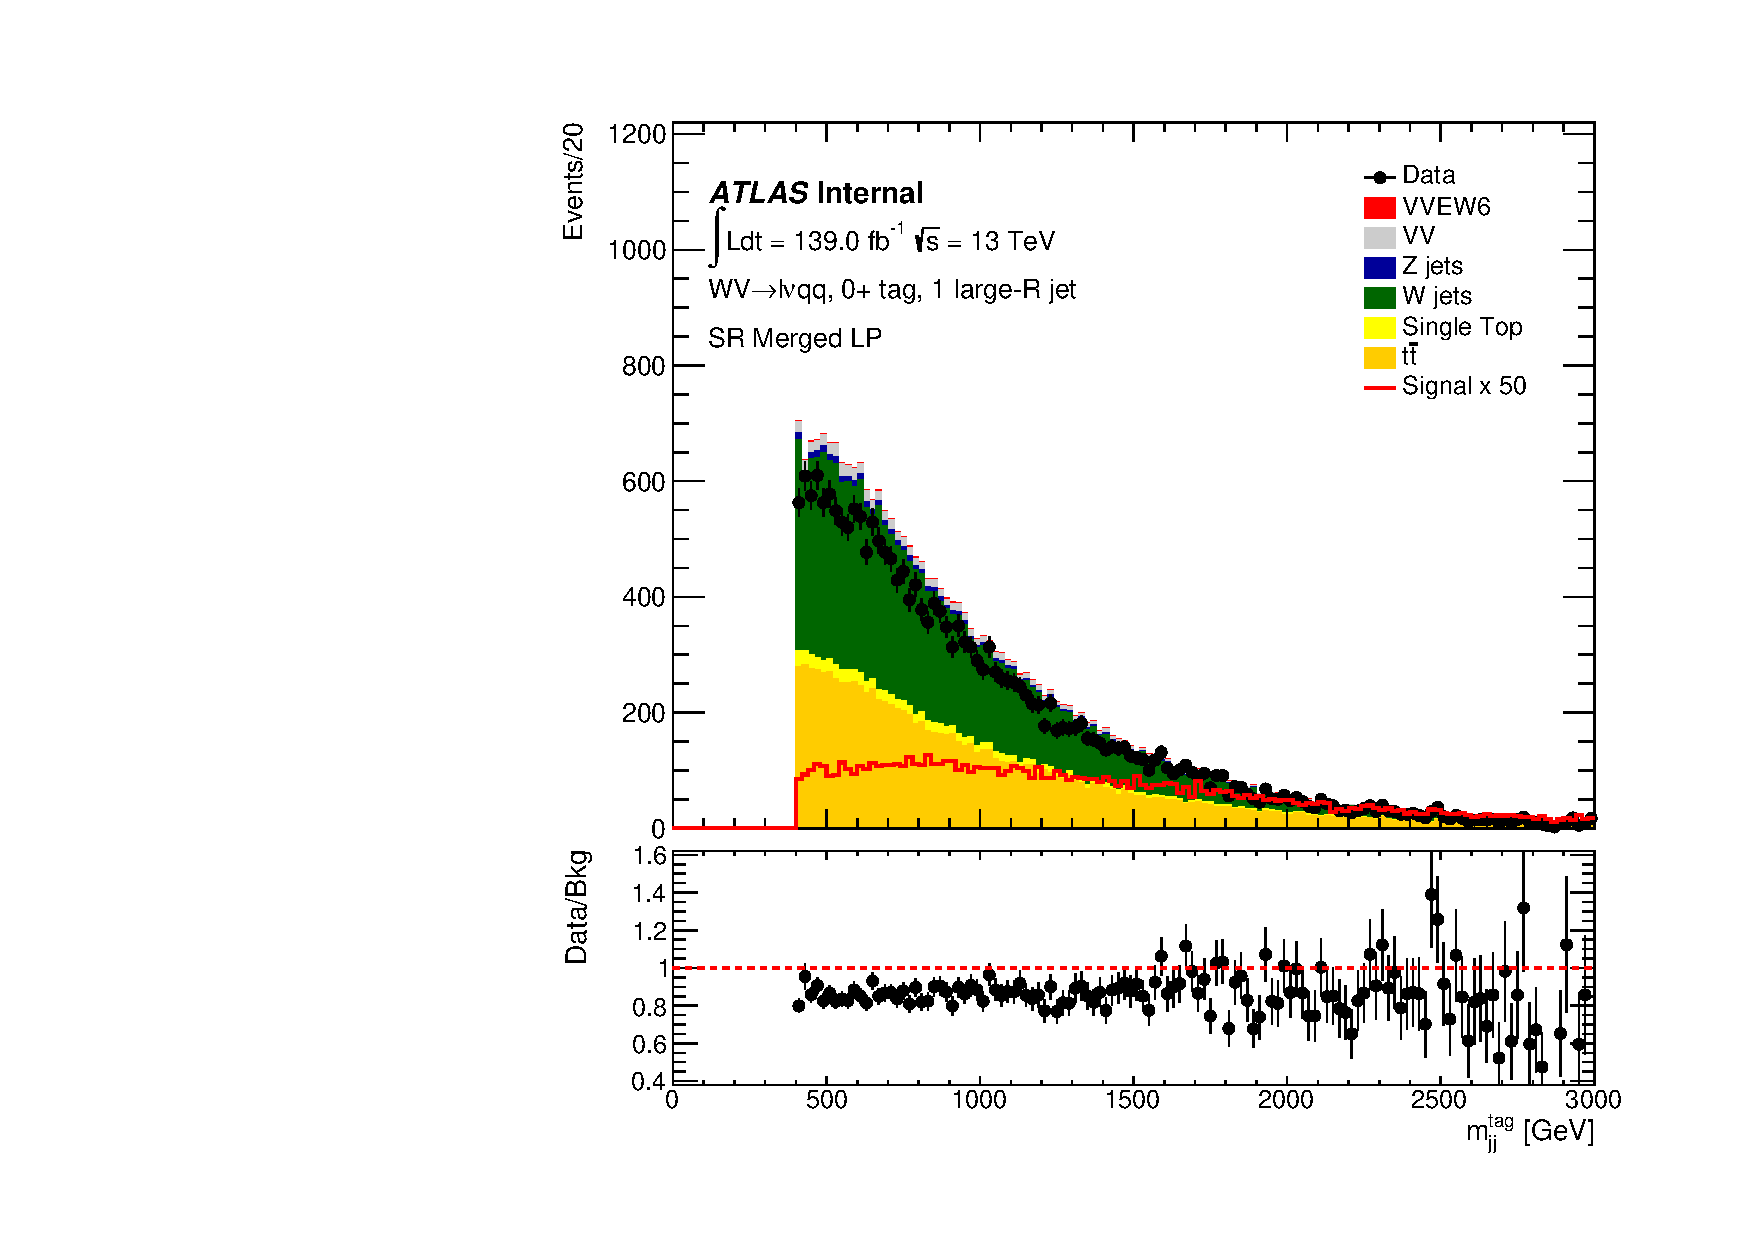
\includegraphics[width=\textwidth]{figures/mjjreweight1lep/SR_80/stacked_plot_merged_tagMjj.pdf}
        \caption{Merged LP SR}
        \label{fig:MC16ADE_Merged_LP_SR}
    \end{subfigure}
    \hfill
    \begin{subfigure}[b]{0.3\textwidth}
        \centering
        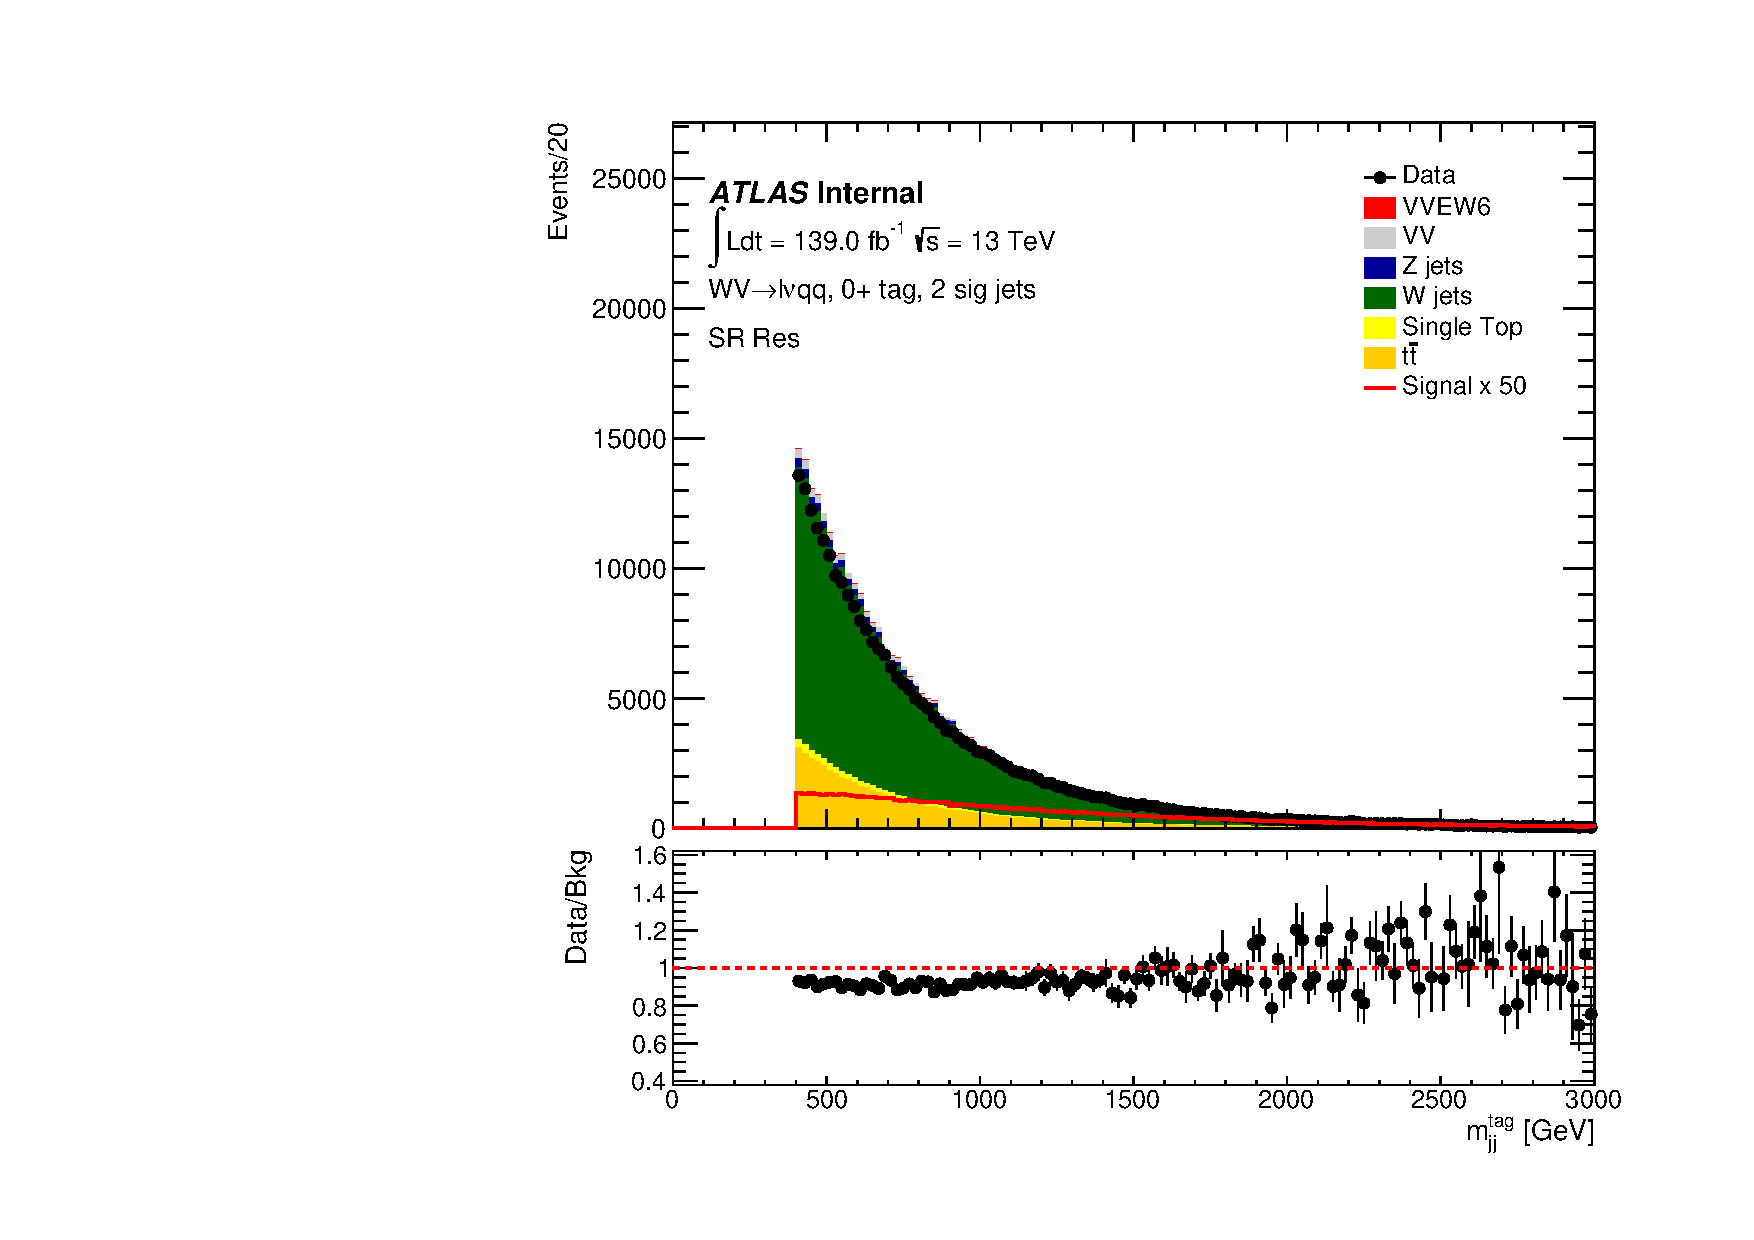
\includegraphics[width=\textwidth]{figures/mjjreweight1lep/SR_Res/stacked_plot_resolved_tagMjj.pdf}
        \caption{Resolved SR}
        \label{fig:MC16ADE_Resolved_SR}
    \end{subfigure}
    \caption{\mjjtag distributions after applying reweighting in the signal regions.}
    \label{fig:mjjReweight1LepMjjDistAfter}
\end{figure}

%%%\begin{figure}[ht]
%%%    \centering
%%%    \begin{subfigure}{0.7\textwidth}
%%%        \centering
%%%        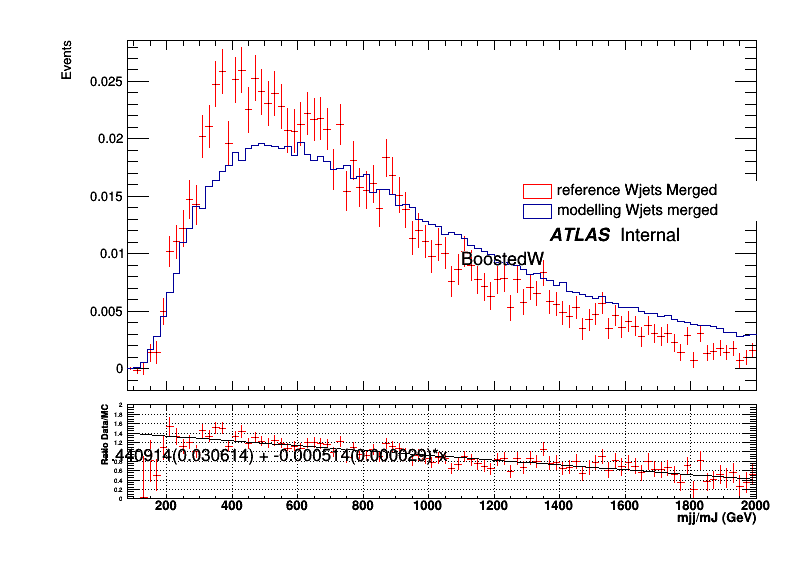
\includegraphics[width=\textwidth]{figures/mjjreweight1lep/merged_WjetsAllMC16T.png}
%%%        \caption{Fit of \(\mjjtag\) slope in merged region, for the entire \(M_J\) range.}
%%%        \label{fig:mjjReweight1LepMer}
%%%    \end{subfigure}
%%%\end{figure}

\begin{figure}[ht]
    \centering
    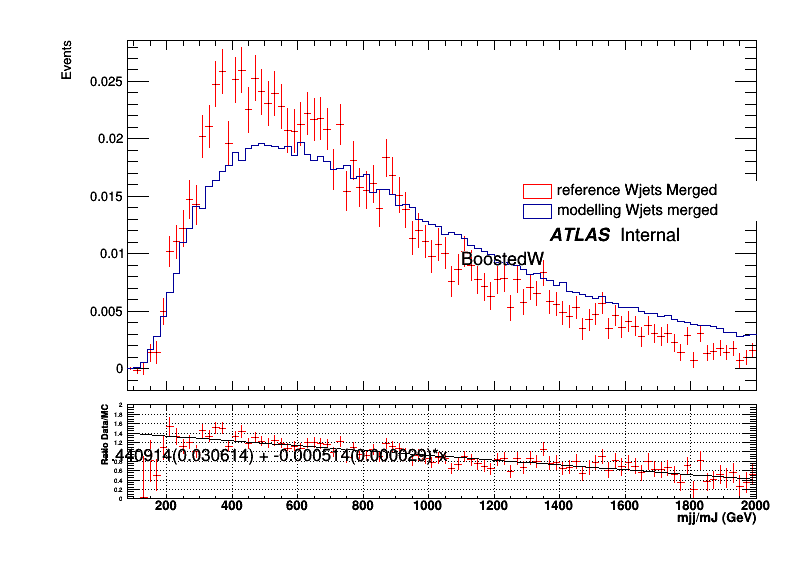
\includegraphics[width=0.7\textwidth]{figures/mjjreweight1lep/merged_WjetsAllMC16T.png}
    \caption{Fit of \mjjtag slope across the full $m_{J}$ range in the merged region.}
    \label{fig:mjjReweight1LepMer}
\end{figure}

\begin{figure}[ht]
    \centering
    \begin{subfigure}[b]{0.3\textwidth}
        \centering
        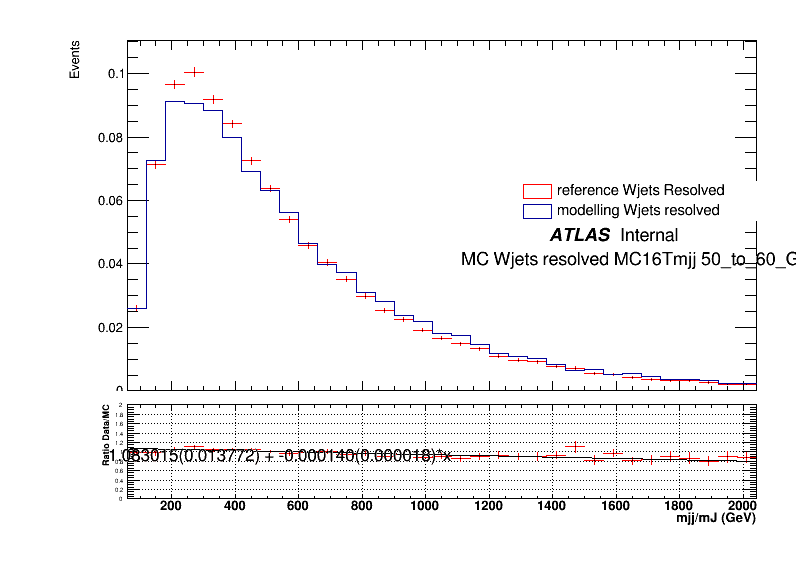
\includegraphics[width=\textwidth]{figures/mjjreweight1lep/resolved_Wjets50_to_60_GeVMC16T.png}
        \caption{50GeV to 60GeV bin}
        \label{fig:resolved_Wjets50to60}
    \end{subfigure}
    \hfill % This will add spacing between the subfigures if needed
    \begin{subfigure}[b]{0.3\textwidth}
        \centering
        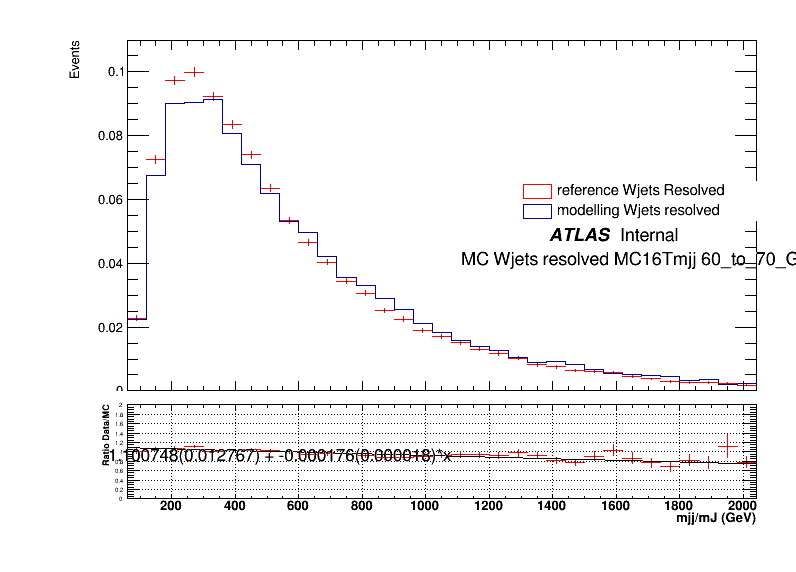
\includegraphics[width=\textwidth]{figures/mjjreweight1lep/resolved_Wjets60_to_70_GeVMC16T.png}
        \caption{60GeV to 70GeV bin}
        \label{fig:resolved_Wjets60to70}
    \end{subfigure}
    \hfill
    \begin{subfigure}[b]{0.3\textwidth}
        \centering
        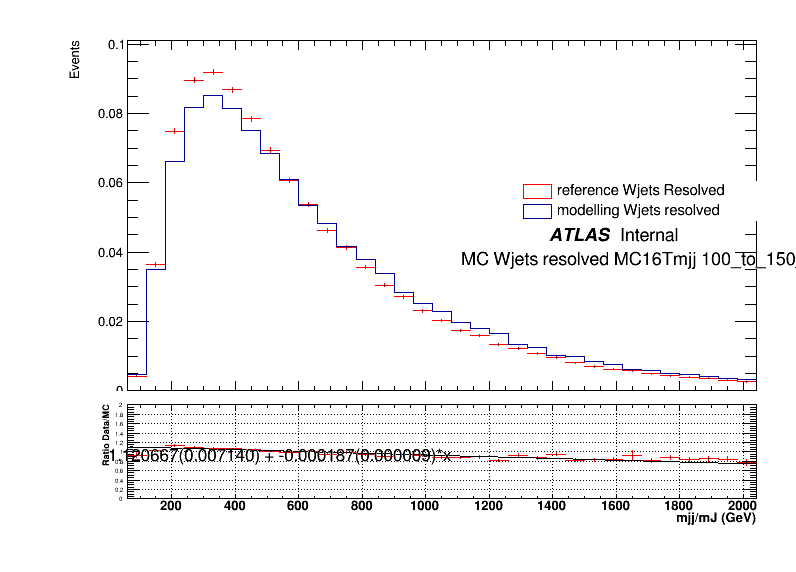
\includegraphics[width=\textwidth]{figures/mjjreweight1lep/resolved_Wjets100_to_150_GeVMC16T.png}
        \caption{100GeV to 150GeV bin}
        \label{fig:resolved_Wjets100to150}
    \end{subfigure}
    
    \begin{subfigure}[b]{0.3\textwidth}
        \centering
        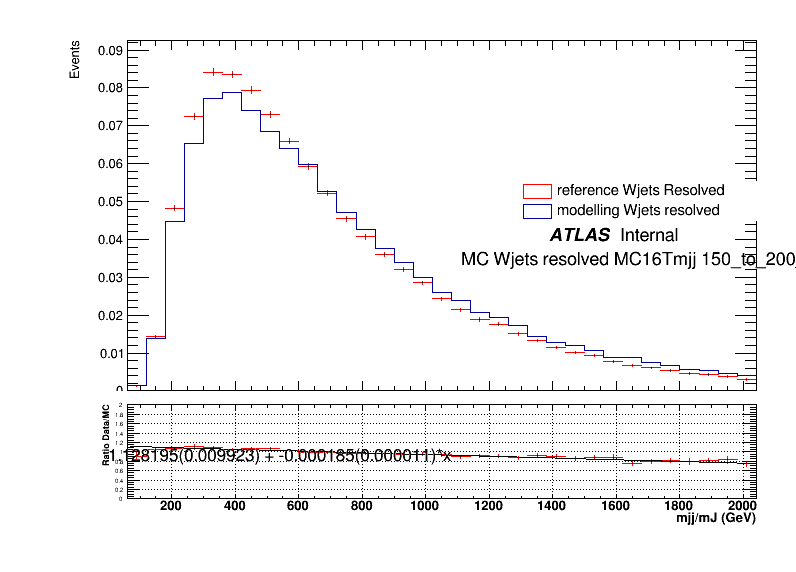
\includegraphics[width=\textwidth]{figures/mjjreweight1lep/resolved_Wjets150_to_200_GeVMC16T.png}
        \caption{150GeV to 200GeV bin}
        \label{fig:resolved_Wjets150to200}
    \end{subfigure}
%    \hfill
    \begin{subfigure}[b]{0.3\textwidth}
        \centering
        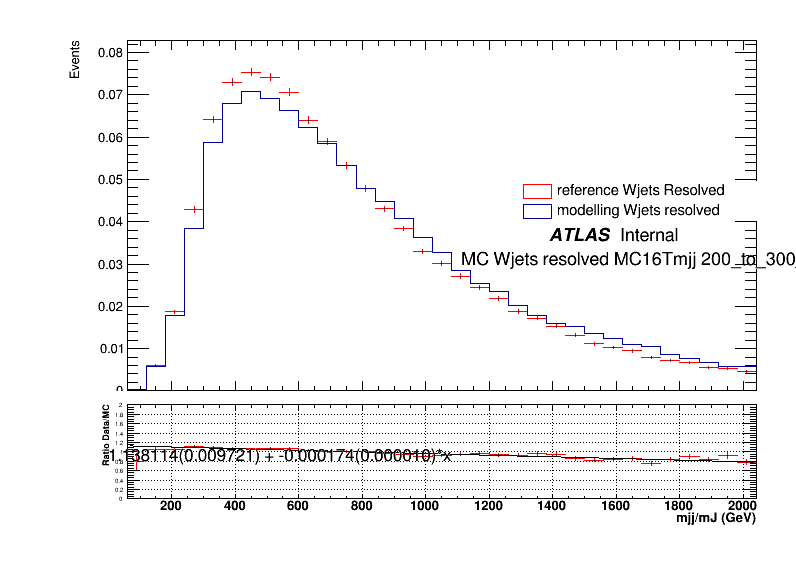
\includegraphics[width=\textwidth]{figures/mjjreweight1lep/resolved_Wjets200_to_300_GeVMC16T.png}
        \caption{200GeV to 300GeV bin}
        \label{fig:resolved_Wjets200to300}
    \end{subfigure}
    \caption{Fit of \mjjtag slope across various $m_{jj}^{sig}$ slices in \Wjets resolved control region.}
    \label{fig:mjjReweight1LepResPtBins}
\end{figure}

\begin{figure}[ht]
    \centering
    \begin{subfigure}[b]{0.45\textwidth}
        \centering
        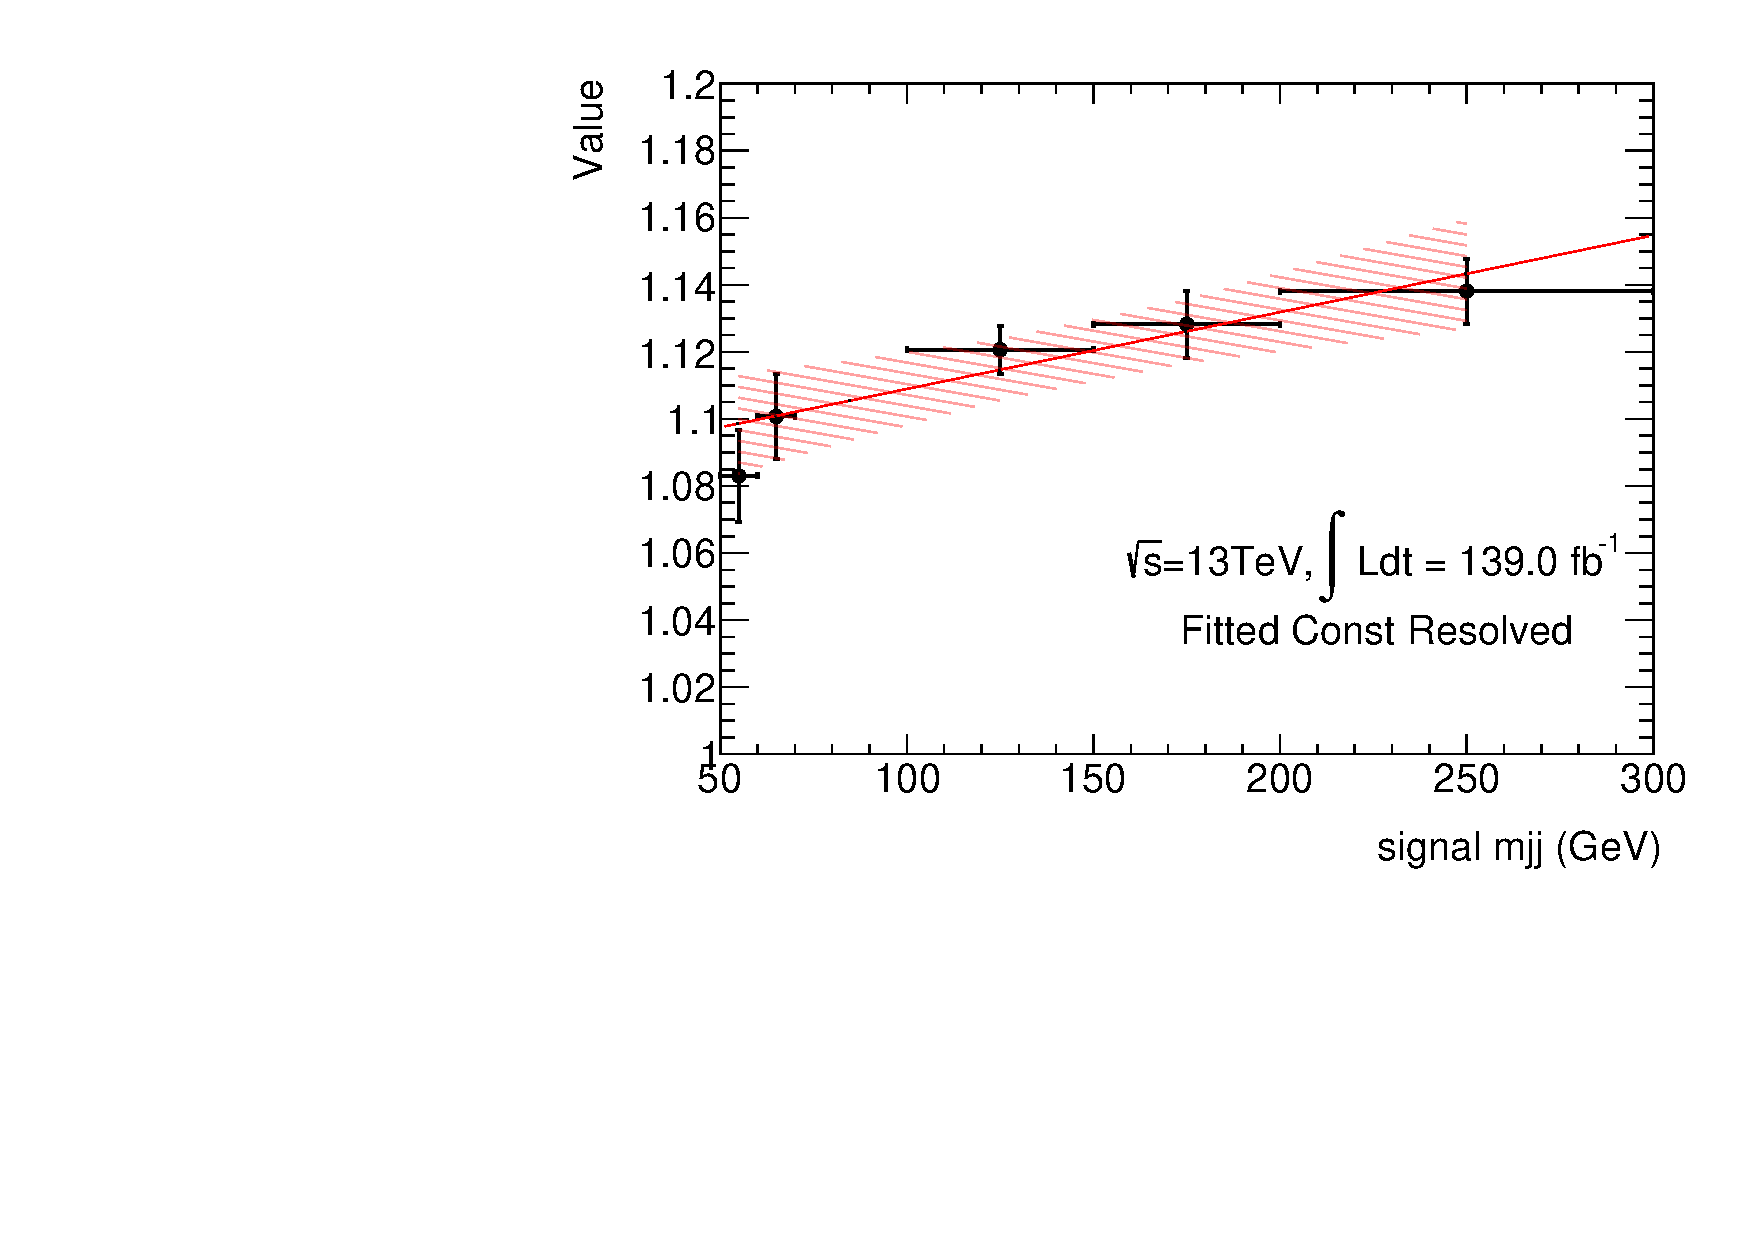
\includegraphics[width=\textwidth]{figures/mjjreweight1lep/fitCResMC16T.pdf}
        \caption{Fit results for ``Constant'', $p_0$.}
        \label{fig:fitCRes}
    \end{subfigure}
    \hfill
    \begin{subfigure}[b]{0.45\textwidth}
        \centering
        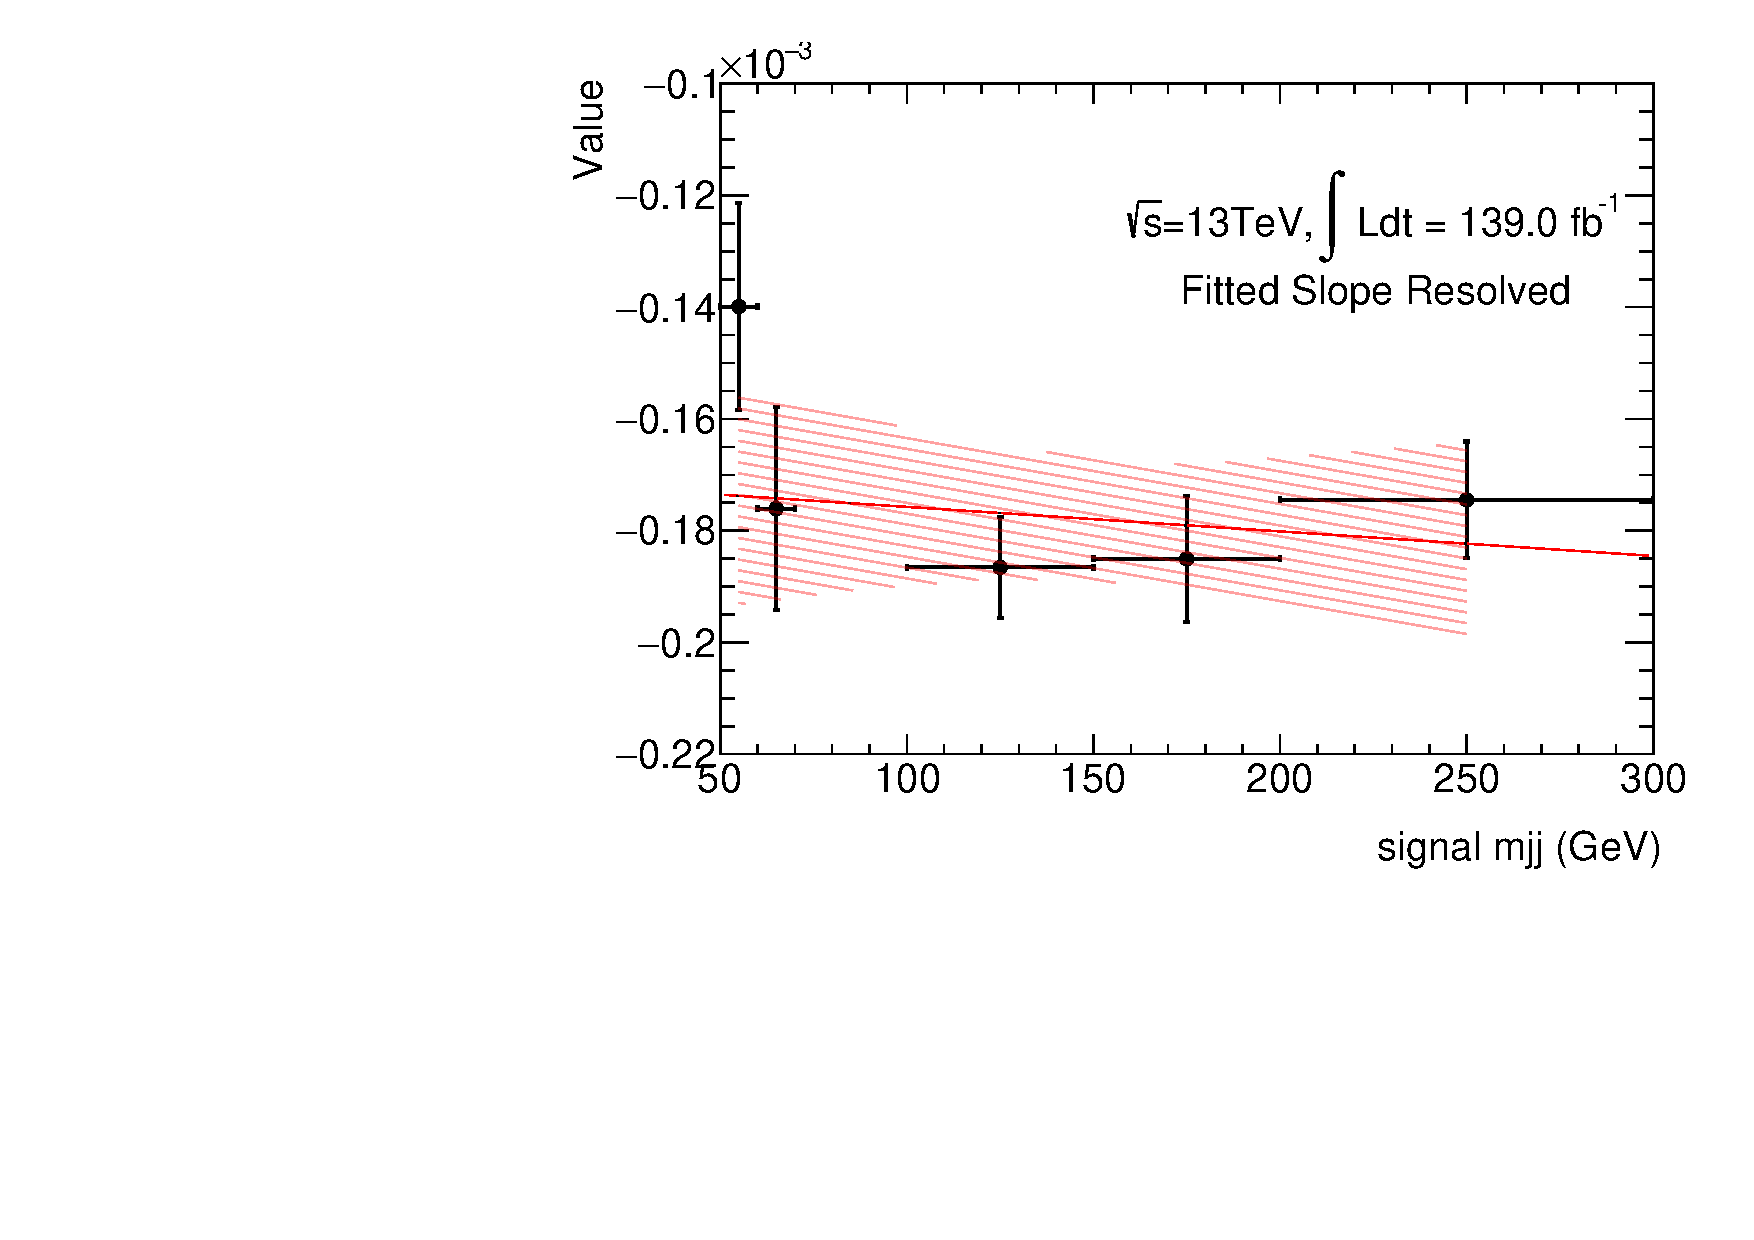
\includegraphics[width=\textwidth]{figures/mjjreweight1lep/fitSResMC16T.pdf}
        \caption{Fit results for ``Slope'', $p_1$.}
        \label{fig:fitSRes}
    \end{subfigure}
    \caption{Slopes and constants as a function of $m_{jj}^{sig}$, with the red band indicating the 68\% confidence level of the fit. 
%The fitted linear function is shown at the top and the fitted result at the signal \(m_{jj}^{sig}\) bin is shown at the bottom.
}
    \label{fig:mjjReweight1LepResFit}
\end{figure}

\begin{figure}[ht]
    \centering
    \begin{subfigure}[b]{0.45\textwidth}
        \centering
        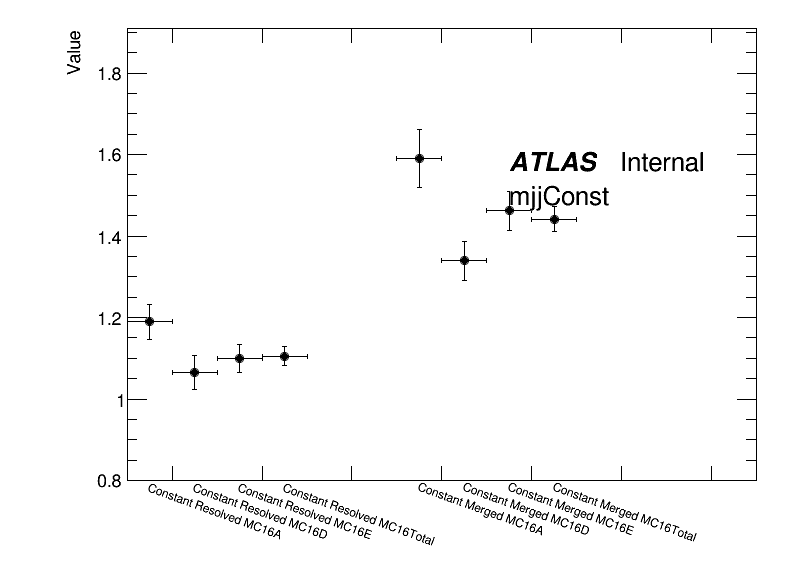
\includegraphics[width=\textwidth]{figures/mjjreweight1lep/TotalConstant.png}
        \caption{Fitted results for ``Constant'', $p_0$.}
        \label{fig:TotalConstant}
    \end{subfigure}
    \hfill
    \begin{subfigure}[b]{0.45\textwidth}
        \centering
        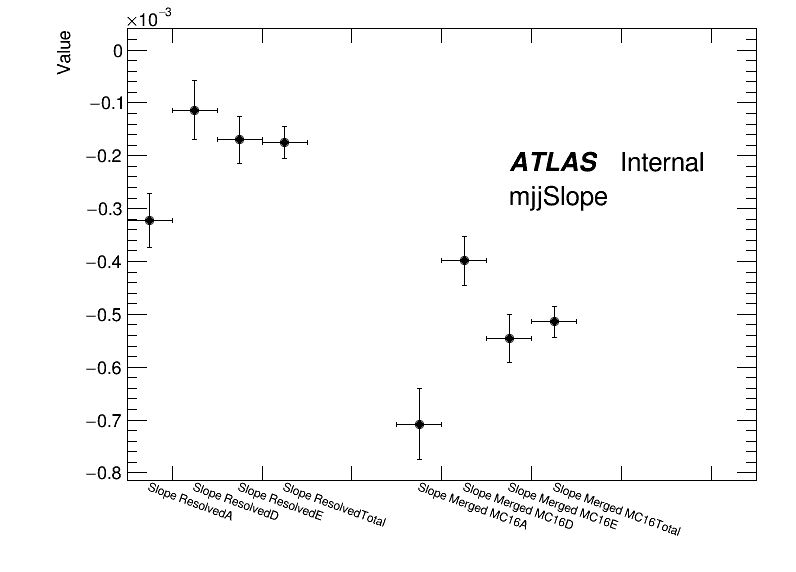
\includegraphics[width=\textwidth]{figures/mjjreweight1lep/TotalSlope.png}
        \caption{Fitted results for ``Slope'', $p_1$.}
        \label{fig:TotalSlope}
    \end{subfigure}
    \caption{Fitted results for slopes and constants for each data period.}
    \label{fig:mjjReweight1LepResTotal}
\end{figure}


